\chapter{\IfLanguageName{dutch}{Stand van zaken}{State of the art}}%
\label{ch:stand-van-zaken}

% Tip: Begin elk hoofdstuk met een paragraaf inleiding die beschrijft hoe
% dit hoofdstuk past binnen het geheel van de bachelorproef. Geef in het
% bijzonder aan wat de link is met het vorige en volgende hoofdstuk.

% Pas na deze inleidende paragraaf komt de eerste sectiehoofding.
\section{\IfLanguageName{dutch}{Wat is er verkeerd met IPv4?}{Wat is er verkeerd met IPv4?}}%
\label{sec:Wat is er verkeerd met IPv4?}


 De meest gebruikte IP versie is vandaag nog altijd IPv4. \autocite{hagen2006ipv6} IPv4 is uitgevonden in de Verenigde Staten in de jaren 70 zodat onderzoekers en overheid met elkaar konden communiceren en informatie uitwisselen. De groep die daar het meest verantwoordelijk voor was, was de Internet Engineering Task Force (IETF).  Het is een van de belangrijkstes instantie die zich bezighoudt met de ontwikkeling van nieuwe internetstandaardspecificaties. Het is geen gebruikelijke organisatie omdat het geen bedrijf is en ook geen raad van bestuur heeft. \autocite{hoffman2006tao} De organisatie is volledig geleid door vrijwilligers die 3 keer per jaar samenkomen om het internet te verbeteren en te standaardiseren. In die tijd hadden de uitvinders nog niet alle nodige fucionaliteiten in het visier. Het protocol diende alleen maar om email en webpaginas te ondersteunen. Ondertussen is er door de exponentiële groei aan netwerktoestellen en complexiteit, nood aan veel meer. De behoefte aan netwerken van vandaag, met name webpagina's, e-mails, peer-to-peer-diensten en het gebruik van mobiele apparaten, is aanzienlijk gegroeid en heeft de verwachtingen van de oorspronkelijke oprichters ruimschoots overtroffen. \autocite{frankel2010guidelines} De vooruitgang van IPv4 was niet genoeg om het protocol in stand te houden. De grootste reden komt door het te kort aan IPv4 adres ruimte. In theorie heeft IPv4, 4.3 miljard IP-adressen. Bij het onstaan van IPv4 werd de beschikbare ruimte als meer dan voldoende beschouwd. Er is nu een tekort ontstaan door de ontoereikende verdeling van de beschikbare ruimte. \textcite{hagen2006ipv6} verklaart in haar paper dat het herverdelen van de bruikbare ruimte niet praktisch is.  \textcite{loshin2004ipv6} verklaart in zijn boek dat het IETF zijn best gedaan heeft om de levensduur van IPv4 te verlangen, maar als het internet wil blijven groeien dat het tijd is voor een nieuw internet protocol.

\section{\IfLanguageName{dutch}{Hoe kan je de problemen van IPv4 oplossen?}{Hoe kan je de problemen van IPv4 oplossen?}}%
\label{sec:Hoe kan je de problemen van IPv4 oplossen?}
Network Addres Transalation (NAT) werd ingevoerd als een tijdelijke oplossing om het te kort aan adresruimte op te vangen. (hagen2006ipv6 ) Verklaart dat dit komt omdat de volgende generatie , namelijk IPv6, nog niet op punt stond. NAT is het mappen van een privaat IP-adres aan een public IP-adres (rajamohandesign). NAT zorgt voor veel meer flexibiliteit. NAT wordt tot vandaag veel gebruikt in \newline IPv4-netwerken ondanks de vele nadelen dat het met zich meebrengt. Deering verwijst hierbij naar onderstaande problemen \autocite{deering2000ipv6}:

\begin{itemize}
    \item	NAT zorgt voor problemen bij de meeste huidige IP-multicast- en IP-mobiliteit Protocollen 
    \item	NAT zorgt voor problemen bij veel bestaande applicaties  
    \item	NAT beperkt de markt voor nieuwe toepassingen en diensten
    \item	NAT brengt de prestaties, robuustheid, veiligheid en beheerbaarheid van het internet naar beneden
\end{itemize}
Men kan zich de vraag stellen “Waarom verbeteren we niet gewoon de gebreken van NAT?”. \textcite{deering2000ipv6} heeft een antwoord hiervoor.Hoewel NAT nog steeds nuttig kan zijn in bepaalde situaties, biedt IPv6 een duurzamere oplossing om de fundamentele beperkingen van IPv4 aan te pakken en te voldoen aan de groeiende eisen van het hedendaagse internet. Verder schrijft hij dat dit alleen maar de complexiteit zal verhogen. Bovendien komen er extra gebreken bovenop. In plaats daarvan is IPv6 ontworpen om een overvloed aan unieke adressen te bieden, waardoor het internet kan blijven groeien zonder uitgebreide NAT-implementaties. IPv6 biedt talloze voordelen, zoals vereenvoudigde netwerkconfiguratie, verbeterde beveiligingskenmerken en ondersteuning voor opkomende technologieën zoals Internet of Things (IoT)-apparaten. \autocite{huston2000nat}

\section{\IfLanguageName{dutch}{De weg naar IPv6}{De weg naar IPv6?}}%
\label{sec:De weg naar IPv6?}

\textcite{bilski2011ipv4} verklaart in zijn paper dat de evolutie van IPv4 naar IPv6 de grootste transformatie is in de structuur van het internet sinds het bestaan. Het is wel een transitie die nodig is. Zo zou de verandering van het aantal adres bits van 32 naar 64 in IPv6 ervoor zorgen dat er in theorie 3 miljard adressen per persoon op de aarde zijn. \textcite{andress2005ipv6} legt in zijn artikel uit dat de grote marge voor IP-adressen niet zo bedoeld is. Veel van de adresbits worden minder efficiënt gebruikt om het configureren van adressen te vergemakkelijken. Er zijn zeker nog genoeg adressen vrij voor gebruik in de toekomst. \autocite{andress2005ipv6} Dit zorgt er ook voor dat IPv6 geen vervolg is op IPv4. IPv6 is een geheel nieuw protocol. 

\section{\IfLanguageName{dutch}{De problemen met IPv6}{De problemen met IPv6?}}%
\label{sec:De problemen met IPv6?}

\subsection{Header manipulation}
In zijn paper waarschuwt \textcite{sotillo2006ipv6} voor het gevaar van header manipulation. Gelukkig kunnen extension headers en IPsec implementaties helpen bij het voorkomen van veel header manipulation aanvallen.Een van de belangrijkste zorgen bij het manipuleren van headers is het potentieel compromitteren van de integriteit van pakketten. IPv6-headers bevatten cruciale informatie die nodig is voor het juist afleveren van pakketten. Wanneer deze headers worden gemanipuleerd, kan de integriteit van de pakketten in gevaar komen. Dit kan leiden tot onjuiste aflevering, wat uiteindelijk netwerkcommunicatie verstoort en potentiële serviceonderbrekingen veroorzaakt. \autocite{dawood2012ipv6} Een ander significant risico dat gepaard gaat met het manipuleren van headers is adresvervalsing. Door de bron- of bestemmingsadressen binnen IPv6-headers te wijzigen, kunnen aanvallers identiteiten vervalsen of legitieme hosts imiteren. Deze kwaadaardige activiteit kan ernstige gevolgen hebben, waardoor aanvallers beveiligingsmaatregelen kunnen omzeilen, ongeautoriseerde acties kunnen uitvoeren of zich kunnen bezighouden met verschillende vormen van cyberaanvallen.
Bovendien kan headermanipulatie ook de exploitatie van netwerkbeveiligingslekken vergemakkelijken. Door bepaalde velden in de headers te manipuleren, kunnen aanvallers mogelijk zwakke plekken in netwerkprotocollen benutten, wat kan leiden tot ongeautoriseerde toegang, informatie lekken of zelfs volledige netwerkcompromissen. geen\autocite{6726061}

\subsection{Multicast adressen}    
Volgens \textcite{1619968} kunnen nieuwe features zoals multicastadressen problemen veroorzaken. De nieuwe types ICMPv6-berichten en de afhankelijkheid van multicastadressen in IPv6 leiden tot nieuwe manieren van misbruik bij flooding attacks. Hoewel ICMPv6-berichten nodig zijn voor een goed functionerend netwerk, moeten ze altijd worden toegestaan in het netwerk. \autocite{DURDAGI20105285} Dit betekent dat error notificatie berichten ook naar multicast-adressen in het netwerk kunnen worden verzonden, wat misbruikt kan worden door hackers. Hierbij zenden hackers een pakket met een error notificatie bericht naar een multicastadres, zodat ze meerdere berichten gericht op één slachtoffer kunnen sturen.

\subsection{TCP}
Een flooding aanval kan ook via het Transmission Control Protocol (TCP) worden uitgevoerd. \autocite{gao2014detecting} In hun paper leggen \textcite{gao2014detecting} uit hoe een dergelijke aanval werkt. Het aanvallende apparaat kan vervalste SYN-verzoeken sturen met een vervalst bronadres naar een slachtoffer. Het slachtoffer stuurt vervolgens een SYN/ACK-antwoord, maar omdat het bronadres vals is, komt er geen ACK terug. Dit kan leiden tot een overbelasting van de verbindingswachtrijen en de geheugenbuffer, waardoor de service voor legitieme TCP-gebruikers wordt geweigerd. \autocite{gao2014detecting} Dit zorgt er dus voor dat de client geen connectie kan maken met de server. Dit is een denial of service (DoS) aanval. \autocite{morbitzer2013tcp} De afbeelding in \ref{fig:SYNflood} is een vereenvoudiging van hoe SYN-flooding aanvallen in de echte wereld plaatsvinden en is bedoeld om alleen het basisidee achter deze soorten aanvallen te begrijpen. \autocite{eddy2006defenses}

\begin{figure}[H]
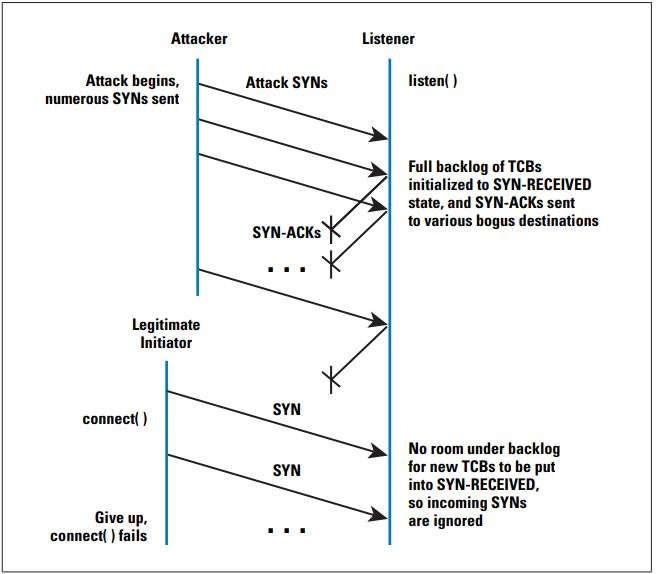
\includegraphics[scale=0.7]{SYNflood.jpg}
\caption{Voorbeeld van SYN-flood aaanval \autocite{eddy2006defenses} }
\label{fig:SYNflood}
\end{figure}  
 
\subsection{Neighbor Discovery}
In het IPv6-protocol is een ander kwetsbaar protocol het Neighbor Discovery (ND) protocol. Dit protocol wordt door apparaten binnen een netwerk gebruikt om informatie over de lokale topologie te verkrijgen, zoals IP- en MAC-adressen, evenals de IP-naar-MAC-mapping van aanwezige routers in het lokale netwerk. \autocite{nikander2004ipv6} Wat dit protocol risicovol maakt, is dat elk apparaat in het netwerk zichzelf kan presenteren als een router. \autocite{ullrich2014ipv6} Hierdoor ontstaat een potentiële mogelijkheid voor een hacker om een routeraankondiging te vervalsen. Deze vervalsing van de routeraankondiging kan ernstige gevolgen hebben voor het netwerkverkeer en de beveiliging ervan. Het kan leiden tot verkeerde routerselectie, waarbij pakketten worden doorgestuurd naar een valse router in plaats van de legitieme router, wat kan resulteren in packet loss of zelfs het mogelijk maken van man-in-the-middle-aanvallen. Bovendien kan het manipuleren van de time to live (TTL) van de router de normale routering van pakketten verstoren en de communicatie binnen het netwerk verstoren.


\subsection{Mobiliteit}
Mobiliteitsondersteuning direct in het protocol zelf integreren was een van de voornaamste doelstellingen van IPv6, in tegenstelling tot IPv4, waarbij gebruik wordt gemaakt van extensies zoals Mobile IP die mogelijk niet naadloos samengaan met onderliggende mechanismen.\autocite{ELGOARANY200732} Op gelijke wijze worden aanvullende beveiligingsextensies zoals IPsec en HTTPS vereist om beveiligingsproblemen aan te pakken bij IPv4, terwijl IPv6 streeft naar directe integratie van beveiligingskenmerken in het protocol.\autocite{sotillo2006ipv6} Mobiliteit maakt gebruik van twee soorten adressen: een permanent adres en een mobiel adres. Het permanente adres is een typisch IPv6-adres, terwijl het mobiele adres een tijdelijk adres is dat wordt gebruikt in de IP-header. Het mobiele adres kan kwetsbaar zijn voor spoofing-aanvallen. Netwerkbeheerders moeten zich bewust zijn van de complexiteit van mobiliteit en speciale veiligheidsmaatregelen toepassen.




\section{\IfLanguageName{dutch}{Mitigatie van IPv6}{De weg naar IPv6?}}%
\label{sec:De weg naar IPv6?}

\subsection{Header manipulation}
\textcite{boek1} leggen in hun boek uit ongeoorloofde pogingen tot headermanipulatie kunnen beperkt worden door het afdwingen van beveiligde netwerkconfiguraties. Dit omvat het configureren van netwerkapparaten en routers met strikte toegangscontrolelijsten (ACL's) en correcte filterregels. Op deze manier wordt ervoor gezorgd dat alleen legitiem en verwacht verkeer toegestaan wordt in het netwerk. Het scannen van een volledig IPv6-segment blijft een aanzienlijke tijdsinspanning vereisen, ondanks het gebruik van 64 bits voor IPv6-adressen, wat resulteert in een veel grotere adresruimte dan IPv4. Aanvankelijk lijkt het een onmogelijke taak om elk individueel adres te scannen, gezien de 2\^64 mogelijke unieke adressen. Zelfs met geavanceerde scantechnieken en enorme rekenkracht kan het doorlopen van elk adres in een volledig IPv6-segment tot wel 580 miljard jaar duren. \autocite{boek1} Het gebruik van de langere adresruimte betekent dus niet automatisch dat IPv6 veilig is. Er kan nog steeds gescanned worden met extra methoden die het taak minder intersief maken. Zo kan het netwerk kan nog steeds het slachtoffer worden van een flooding attack.

\subsection{Multicast adressen} 

Het beveiligen van multicast is historisch gezien een uitdaging vanwege de aard ervan. Het multicast-model omvat een enkele bron die naar meerdere ontvangers stuurt, waardoor het moeilijk is om traditionele beveiligingsmaatregelen toe te passen. \autocite{6726061} Toch is het mogelijk om deze aanvallen in IPv6 te verminderen, stelt \textcite{deering2000ipv6} dat een ICMPv6-bericht niet gegenereerd mag worden als reactie op een pakket met een IPv6 \newline multicast-bestemmingsadres, een link-layer multicast-adres of een link-layer \newline broadcast-adres. Aan de andere kant kan de smurf-aanval, zelfs als nodes voldoen aan RFC 2463, gebruik maken van de gegenereerde foutberichten Parameter problem
\newline

ICMPv6 message als reactie op een pakket bestemd voor een multicast-groep \autocite{vyncke2009ipv6}, en kan het pakketten gebruiken die werden gebruikt in een multicast-videostream, omdat multicast-videostream pad maximum transmission unit (MTU) discovery vereist. \textcite{vyncke2009ipv6} stellen dat dit de deur opent naar een amplificatieaanval. Om dit probleem aan te pakken, adviseren ze ook om rate limiting toe te passen op die ICMP-berichten: deze berichten moeten zeldzaam zijn in elk netwerk, zodat een rate limit (10 berichten/seconde) het correcte gebruik van deze berichten (path MTU discovery) kan toestaan, terwijl de amplificatieaanval wordt geblokkeerd. \textcite{6726061} vat het uitstekend samen, het belangrijkste is het waarborgen van de veiligheid van multicast. Het is van essentieel belang voor het succesvol implementeren van groepscommunicatietoepassingen in IPv6. Het beveiligen tegen verkenning, DoS-aanvallen met versterking en het beschermen van het multicast-model zelf zijn cruciale aspecten om mogelijke risico's te verminderen.

\subsection{TCP}
Om te voorkomen dat SYN-Flooding aanvallen plaatsvinden, zijn er verschillende methoden ontwikkeld. \autocite{morbitzer2013tcp} Een van deze methoden zijn SYNCookies. Bij het creëren van een sequentienummer voor het TCP-segment met de SYN- en ACK-vlag maakt de server specifieke keuzes en berekent het sequentienummer op basis van een tijdteller, de Maximum Segment Size (MSS) gekozen door de server en een geheime functie. Dit sequentienummer wordt de SYN-Cookie genoemd.
Een andere methode voor bescherming tegen SYN-Flooding is een SYN-cache. In tegenstelling tot SYN-Cookies wordt informatie over de half-open verbinding nog steeds op de server opgeslagen, maar wordt de hoeveelheid geheugen die nodig is om de verbinding te onthouden geminimaliseerd. Dit wordt gedaan door een hash-waarde op te slaan met informatie over de bron- en bestemmingsadres en -poort en een willekeurig gekozen geheim in plaats van de originele waarden. 
Bovendien verklaart \textcite{morbitzer2013tcp} dat er nog veel meer defensieve technieken zijn zoals het filteren en het vergroten van de backlog queue.


\subsection{Neighbor Discovery}

Een mogelijke oplossing om de beveiliging van Neighbor Discovery-berichten te verbeteren, is de implementatie van Secure Neighbor Discovery (SEND). SEND introduceert nieuwe opties die dit mogelijk maken. \autocite{arkko2005secure} \textcite{7726976} bevestigen in hun paper dat SEND een krachtig mechanisme is om IPv6-link-local communicatie te beveiligen. Hoewel SEND wordt beschouwd als een veelbelovende oplossing om het ND-protocol te beschermen, is de implementatie ervan niet eenvoudig en dus uitdagend.
\newline

Er bestaat nog steeds de mogelijkheid om te spoofen in een IPv6-netwerk. \autocite{1333418} Neighbor Discovery zorgt ervoor dat spoofing alleen mogelijk is bij toestellen in hetzelfde netwerksegment. Dit geldt echter niet voor een 6to4 transitienetwerk. Omdat dit netwerk gebruikmaakt van protocol-encapsulatie, kunnen er andere problemen optreden, zoals adres-spoofing. Als dit het geval is, wordt er een gespoofd adres gebruikt om het interne netwerkpakket te maskeren. \autocite{1333418}

\subsection{Mobiliteit}


Het bewustzijn van de inherente complexiteit van mobiliteit in netwerken is van essentieel belang voor netwerkbeheerders, vooral in het geval van IPv6. Het beheer van de mobiliteit van apparaten en het waarborgen van hun veiligheid vormen cruciale verantwoordelijkheden voor deze beheerders. \textcite{aura2006designing} omschrijven dat mobiliteit uitdagingen met zich meebrengt op het gebied van netwerkbeveiliging, waarbij het behoud van de vertrouwelijkheid, integriteit en beschikbaarheid van gegevens tijdens de verplaatsing van apparaten tussen diverse netwerken en locaties centraal staat.
\newline

Om deze uitdagingen succesvol aan te pakken, dienen netwerkbeheerders speciale veiligheidsmaatregelen te implementeren. Dit omvat het toepassen van beveiligingsmechanismen zoals IPsec (Internet Protocol Security) om de vertrouwelijkheid en integriteit van gegevens te waarborgen gedurende de overdracht tussen mobiele apparaten en netwerken. Daarnaast is het van belang dat netwerkbeheerders zich richten op het effectieve beheer van gebruikersidentiteiten en de implementatie van authenticatieprotocollen, zodat uitsluitend geautoriseerde gebruikers toegang krijgen tot het netwerk.


\section{\IfLanguageName{dutch}{IPv6 Toolkit}{IPv6 Toolkit}}%
\textcite{gont2013security} verklaren dat de introductie van hun "SI6 Networks' IPv6 Toolkit", gebruikers momenteel een alternatieve mogelijkheid bieden om hun \newline IPv6-netwerken te beveiligen en problemen op te lossen, waardoor een eerdere afhankelijkheid van THC's IPv6-AttackSuite doorbroken wordt. Deze toolkit heeft tot doel een uitgebreide beveiligingsanalyse en probleemoplossing te bieden voor IPv6-netwerken en implementaties, waarbij speciale aandacht wordt besteed aan de ontwikkeling van schone, draagbare en veilige code. Daarnaast is er een aanzienlijke inspanning geleverd om gebruikers te voorzien van gedegen documentatie ter ondersteuning van hun IPv6-beveiligingsactiviteiten.
\newline

Een opmerkelijk kenmerk van SI6 Networks' IPv6 Toolkit is dat het vrij beschikbaar is als open source software, waardoor het toegankelijk is voor een breed scala aan gebruikers die geïnteresseerd zijn in IPv6-beveiliging, ongeacht hun financiële mogelijkheden. Dit biedt de gebruikers de gelegenheid om te profiteren van de opgedane expertise en het toegewijde werk op het gebied van IPv6-beveiliging door SI6 Networks.
\newline

De twee auteurs van de IPv6 Toolkit zijn Fernando Gont en Marc Heuse. 
Fernando Gont is een zeer ervaren beveiligingsonderzoeker en consultant bij SI6 Networks. Met zijn expertise heeft hij uitgebreide beveiligingsbeoordelingen uitgevoerd op verschillende communicatieprotocollen. Een opmerkelijk aspect van de carrière van Fernando Gont is zijn actieve deelname aan de IETF. Als betrokken lid van deze invloedrijke organisatie heeft hij zijn kennis en inzichten bijgedragen aan de ontwikkeling en standaardisatie van internetprotocollen. \autocite{gont2013security} Zijn werk binnen de IETF getuigt van zijn toewijding om de beveiliging en betrouwbaarheid van netwerkinfrastructuren te verbeteren. Door samen te werken met andere experts in het veld heeft Fernando Gont een belangrijke rol gespeeld bij het stimuleren van vooruitgang op het gebied van netwerkbeveiliging.
Marc Heuse is een bekende onafhankelijke security-onderzoeker en consultant. Een opmerkelijke prestatie van Marc Heuse is zijn rol als oprichter van The Hacker's Choice . Dit platform getuigt van zijn expertise en passie voor het verkennen en verbeteren van beveiligingsmaatregelen. Naast zijn bijdragen als onderzoeker en consultant wordt Marc Heuse ook erkend als auteur van talrijke publieke beveiligingstools. Deze tools, waaronder thc-ipv6, hydra, amap, THCScan, SuSEfirewall 1 + 2 en vele anderen. \autocite{gont2013security}
Door het  werk van de beide auteurs hebben ze  een toewijding aan het bevorderen van het vakgebied cybersecurity laten zien. Hun uitgebreide ervaring en diverse vaardigheden hebben hun gevestigd als een betrouwbaar figuren in de branche, en hun bijdragen blijven een aanzienlijke impact hebben op de ontwikkeling en verbetering van beveiligingsmaatregelen.


